\section{Probleme}
\label{cha:Probleme}
Das folgende Kapitel beschäftigt sich mit den Problemen, die während der Implementationsphase aufgetreten sind und wie diese gelöst wurden. Hauptsächlich waren dies Probleme mit der Kinect, der Halterung der Weitwinkelkamera, der Belichtungswerte und des Fahrwerks.

\subsection{Kinect - unnatürliche Farben}
\label{sec:farben}
Die Kamera der Kinect hat eine unnatürliche Farbdarstellung.
Es sind sind starke Unterschiede zwischen Kamerabild und der Wirklichkeit zur erkennen.

\begin{figure}[ht]
	\centering
	\begin{subfigure}{0.45\textwidth}
		\centering
		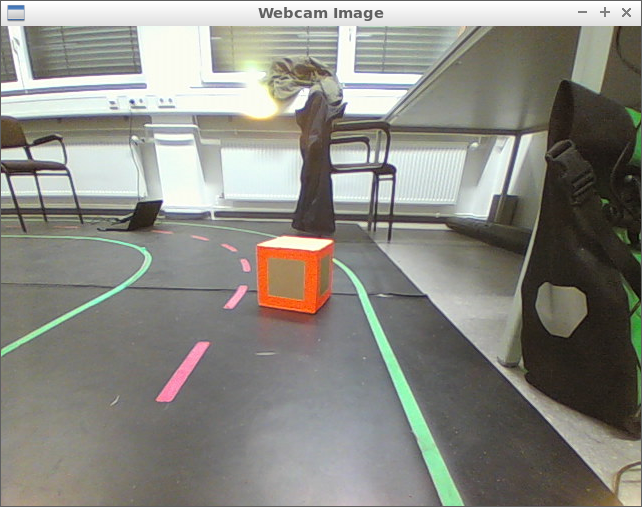
\includegraphics[width=0.9\textwidth]{images/Webcam_RAW.png}
		\caption{Webcam Original}
	\end{subfigure}
	\begin{subfigure}{0.45\textwidth}
		\centering
		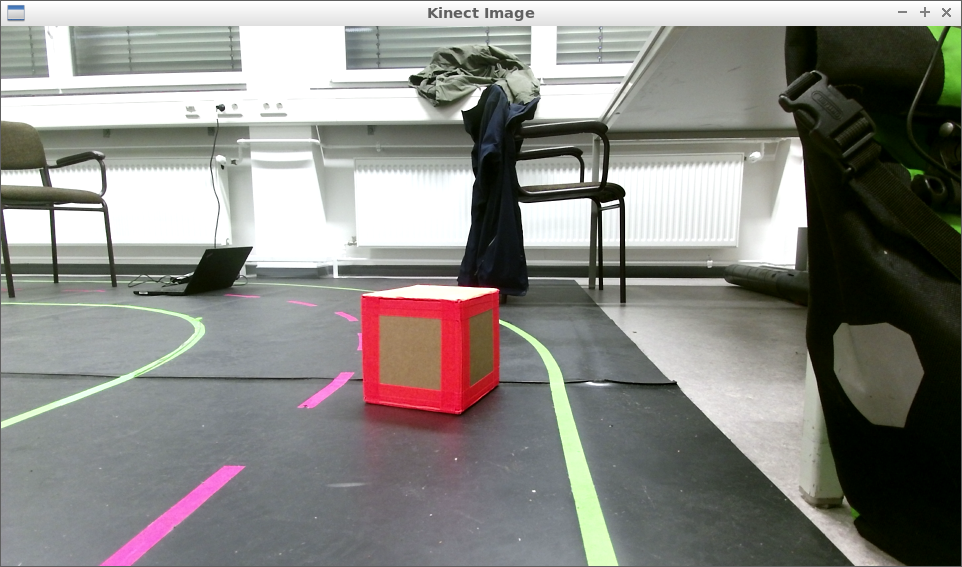
\includegraphics[width=0.9\textwidth]{images/Kinect_qHD_RAW.png}
		\caption{Kinect Original}
	\end{subfigure}
	\caption{Farbdarstellung von Webcam und Kinect}
\end{figure}

Die Farben der Kinect sind übersaturiert und haben teilweise nicht einmal den richtigen Farbton.

\subsection{Kinect - kleines Sichtfeld}
\label{sec:sichtfeld}
Das Sichtfeld der Kinect Kamera fällt relativ klein aus.
Das hat auch damit zu tun, dass die Kinect in einem Winkel auf dem Fahrzeug angebracht ist, mit dem das Sichtfeld erst circa 30cm vom Fahrzeug entfernt beginnt.
Dadurch kann der Abstand des Fahrzeuges zur Fahrbahnbegrenzung zum aktuellen Zeitpunkt nicht ohne weiteres bestimmt werden. 
Zudem ist die Kamera in der Kinect am rechten Rand platziert.
Dadurch ist die linke Fahrbahnbegrenzung häufig nicht im Sichtfeld.
Dieser Effekt wird noch durch die Transformation zum Bird-Eye View verstärkt.

\begin{figure}[ht]
	\centering
	\begin{subfigure}{0.45\textwidth}
		\centering
		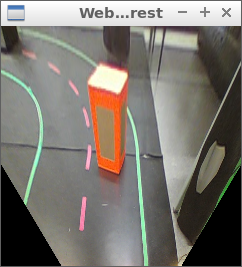
\includegraphics[width=0.9\textwidth]{images/Webcam_BirdEye_ROI.png}
		\caption{Webcam Bird-Eye View und Bildausschnitt}
	\end{subfigure}
	\begin{subfigure}{0.45\textwidth}
		\centering
		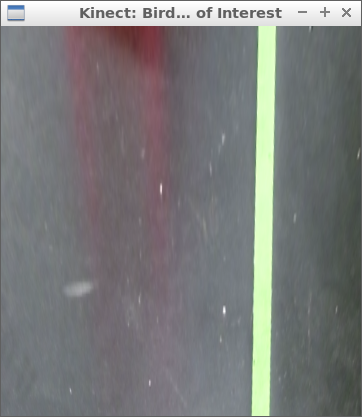
\includegraphics[width=0.9\textwidth]{images/Kinect_BirdEye_ROI.png}
		\caption{Kinect Bird-Eye View und Bildausschnitt}
	\end{subfigure}
	\caption{Sichtfeld von Webcam und Kinect}
\end{figure}

Um eine robuste Fahrbahnerkennung zu implementieren, sind ordentliche Ausgangsdaten von großer Wichtigkeit.
In unserem Fall benötigen wir eine natürliche Farbdarstellung, ein ausreichend großes Sichtfeld das möglichst nah am Fahrzeug beginnt und eine flüssige Bildrate. 
Alle diese Anforderungen werden von der Webcam erfüllt.
Die Webcam kann zudem sehr flexibel auf dem Fahrzeug angebracht werden.
\\
Die Halterung der Webcam verursacht allerdings ein weiteres Problem: eine geringfügige Änderung des Kamerawinkels hat merkliche Auswirkungen auf die Transformation zum Bird-Eye View.
Wenn der Bird-Eye View nicht mehr korrekt berechnet wird, funktioniert die Erkennung der Fahrsituation nicht mehr so gut.
Genauer wird nicht mehr erkannt, wann sich das Fahrzeug auf einer Geraden befindet.
Da die Regelung abhängig von der Fahrsituation ist, kann das Fahrverhalten erheblich schlechter werden. Eine stabile Befestigung der Webcam ist daher wichtig. Näheres dazu im folgenden Abschnitt.

\subsection{Befestigung der Weitwinkelkamera}
\label{sec:befestigung}
Während die Kinect Kamera fest mit dem Fahrzeug verschraubt ist, stellt sich bei Verwendung der Weitwinkelkamera die Frage nach deren Positionierung und Befestigung. Der mitgelieferte Standfuß kann nicht sinnvoll auf dem Fahrzeug fixiert werden, da er nur für stationären Betrieb geeignet ist. Zudem kommt es durch die Vibrationen im Fahrbetrieb zu einer schleichenden Veränderung des Kamerawinkels mit den in \autoref{sec:sichtfeld} beschriebenen Auswirkungen.
Um eine stabile und auch optisch ansprechende Lösung zu finden, wurde mittels CAD-Software eine Kamerahalterung entworfen und auf einem 3D-Drucker ausgedruckt. Dies bietet gleich mehrere Vorteile:

\begin{itemize}
	\item Die Kameraposition kann frei gewählt werden
	\item Die Halterung ist stabil, aber sehr leicht
	\item Aufgrund des modularen Aufbaus der Halterung ist ein späterer Umbau sehr einfach möglich
	\item Die Kinect Kamera kann demontiert werden, dies entlastet die Vorderachse
\end{itemize}

Die Halterung besteht aus einem unteren Teil zur Befestigung am Fahrzeug, einem Mittelteil der das Emblem der Gruppe zeigt, sowie einem oberen Teil, auf dem die Webcam montiert wird. \autoref{fig:halterung} zeigt das CAD-Modell, der reale Aufbau ist in \autoref{abb:halterung} zu sehen.

\begin{figure}[H]
		\centering
		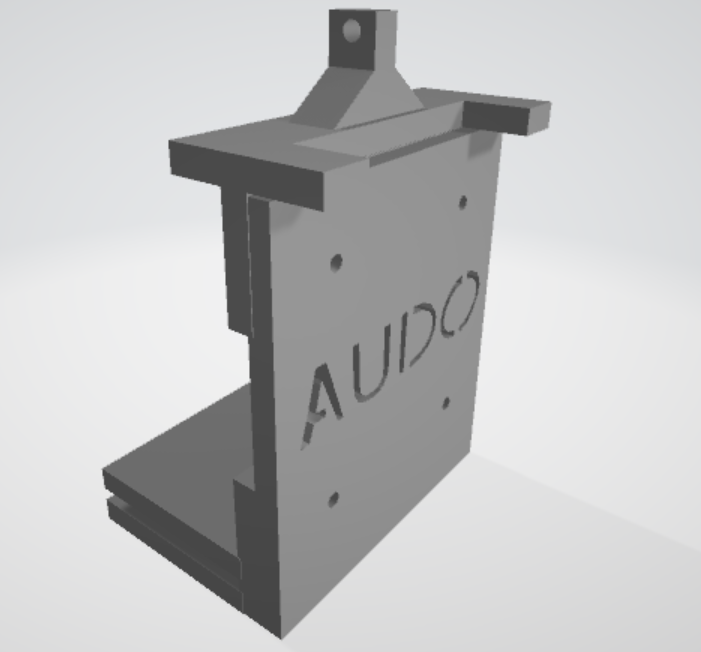
\includegraphics[width=0.5\textwidth]{images/CAD_Halterung.png}
	\caption{3D-Modell der Kamerahalterung}
	\label{fig:halterung}
\end{figure}


\subsection{Weitwinkelkamera verändert Belichtung zur Laufzeit}
\label{sec:belichtung}
Die Weitwinkelkamera passt ihre Belichtung an die aktuellen Lichtverhältnisse zur Laufzeit an.
Das führt leider dazu, dass selbst kleine Veränderungen der Lichtverhältnisse die Belichtung ändern, wie zum Beispiel Lichtspiegelungen auf dem Boden.
Wenn sich die Belichtung ändert, ändern sich auch schlagartig die Farbwerte.
Um keine komplizierte Anpassung der Filterparameter während der Laufzeit vornehmen zu müssen, muss die Belichtung konstant gehalten werden.
Das ist bei dieser Weitwinkelkamera nicht in der Software einstellbar.
Deshalb wurde ein pragmatischer Ansatz gewählt, um dieses Problem zu lösen.
Die Weitwinkelkamera wird mit einer LED Leiste geblendet, welche über das 12V Boardnetz gespeißt wird.
Damit nimmt die Weitwinkelkamera die Umgebung immer sehr hell wahr.
Leichte Veränderungen der tatsächlichen Lichtverhältnisse werden durch das Blenden einfach herausgefiltert. 
Das Ergebnis ist eine konstante Belichtung und somit auch konstante Farbwerte.

\subsection{Fahrwerk}
\label{sec:fahrwerk}
Die Räder kollidieren bei zu hohem Lenkwinkel mit dem Gehäuse.
Deswegen wird der maximale Lenkwinkel auf einen ausgemessenen Wert begrenzt.
\\
Die Lenkmechanik des Fahrzeugs ist aus Plastik und nicht sonderlich genau gefertigt.
Das hat zur Folge, dass die Lenkung ein merkliches Spiel hat. 
Dies bedeutet, dass kleine Veränderungen am Lenkwinkel keine realen Auswirken haben. 
Außerdem liegt relativ viel Last auf der Vorderachse, weil der Akku und die Kinect vorne im Fahrzeug platziert sind.
Dadurch wird die Lenkmechanik noch zusätzlich belastet.
Bei höheren Geschwindigkeiten sollte sich dieser Effekt allerdings abschwächen. 
Durch diese Effekte kann sich nicht darauf verlassen werden, dass nach dem Einstellen eines Lenkwinkels, dieser auch tatsächlich anliegt.
In der Praxis wird allerdings immer mindestens so schnell gefahren, dass dieser Effekt keine allzu großen Auswirkungen hat.
\\
Ein weiteres Problem besteht darin, dass der Lenkwert der an die \code{UC\_Bridge} gesendet wird, sich nicht linear in einen Lenkwinkel umrechnen lässt.
Die Beziehung zwischen Lenkwert und Lenkwinkel auszumessen gestaltet sich schwierig.
Da diese Beziehung stark von der Geschwindigkeit und der Last auf die Lenkmechanik abhängt.
Wenn der tatsächliche Lenkwinkel durch passende Sensoren regelmäßig gemessen werden würde, könnte eine Regelung für den Lenkwinkel konzipiert werden.
Dieses Problem wurde jedoch nicht weiter beachtet, da sich auf eine möglichst robuste Regelung zur Fahrspurhaltung konzentriert wurde und diese das Problem teilweise ausgleichen kann. 
Um die Lenkmechanik nicht unnötig zu belasten, wurde eine möglichst ruhige Regelung implementiert.




